\documentclass[phd]{buptthesis}

\BUPTthesiscntitlepage{%
	title = {北京邮电大学 \\ 博士、硕士论文\LaTeX 模板 \\ 信通院$ \text{IC}^\text{2} $ Laboratory},
	studentid = {2019},
	name = {简单男孩},
	major = {信息与通信工程},
	supervisor = {香\quad \quad 农},
	institute = {信息与通信工程学院},
	degreetype = {工学}}

%% \quad 相当于一个汉字的宽度,同时也相当于~~~~

\BUPTthesisentitlepage{%
	title = {A \LaTeX~TEMPLATE FOR PHD DISSERTATION OF BUPT},
	desc = {A DISSERTATION\\SUBMITTED TO THE FACULTY OF THE GRADUATE\\SCHOOL OF BEIJING UNIVERSITY OF POSTS AND\\TELECOMMUNICATIONS},
	name = {BY\\DOCTOR},
	supervisor = {PROF. SOMEONE, PH.D. ADVISOR},
	major = {INFORMATION AND COMMUNICATIONS ENGINEERING},
	degree = {FOR THE DEGREE OF
		\\ DOCTOR OF PHILOSOPHY IN\\INFORMATION AND COMMUNICATIONS ENGINEERING}
}
\begin{document}

\makechinesetitle
\makeenglishtitle
\makestatement

\frontmatter
\begin{cnabstract}
北京邮电大学博士学位论文\LaTeX 模板

\cnkeywords{\LaTeX~~模板~~北京邮电大学~~博士学位论文}
\end{cnabstract}

\begin{enabstract}
	
\LaTeX~Template

\enkeywords{\LaTeX Template~~BUPT~~PhD~~Dissertation}
\end{enabstract}

\tableofcontents
\listoffigures
\listoftables
%\BUPTlongestlength{nomenclature = { $BUPTBUPTBUPT$ }}
\begin{nomenclature}

	\item[\LaTeX]\hfill \LaTeX

\end{nomenclature}


\mainmatter
\include{Chapter/Chapter_introduction}
\chapter{文字与图表}
\section{文字}
每章的标题以\textbf{三号黑体字}居中打印;“章”下\cemph{空两行}为节的标题,以\textbf{四号黑体字}左起打印;“节”下空一行为小节的标题,以\textbf{小四号黑体字}左起打印。换行后打印论文正文。文字的行间距20磅,字符为标准间距。

\subsection{数值与单位}

单位采用宏包\href{http://mirrors.sjtug.sjtu.edu.cn/ctan/macros/latex/contrib/siunitx/siunitx.pdf}{\textit{siunitx}}插入,例如传输速率是$\SI{100}{\mega\byte}$,信噪比为$\SI{20}{\mdecibel}$。(注意,如果要使用字节单位,则需要增加选项\cemph{binary-units}) 

引用一个表格\ref{chap:notation}。

\section{表}

\begin{table*}[!htb]
	\centering
	\caption{数学符号含义表(标题及序号置于表的正上方)}
	\label{chap:notation}
	\begin{tabular}{|c|c||c|c|}
		\hline
		\rowcolor{LightSteelBlue}
		\textbf{符号} 			& \textbf{含义} 	    & \textbf{符号}		  & \textbf{含义} 		   	 \\
		\hline
		$N$ 					 & 数量		   		 & $\mathbb{N}$ 		 & 集合 						\\
		\hline
		$\gamma$ 				 & 信噪比			    & $\mathcal{T}$ 		& 时刻		 			   \\
		\hline
	\end{tabular}
\end{table*}

\section{图}

\begin{figure}
	\centering
	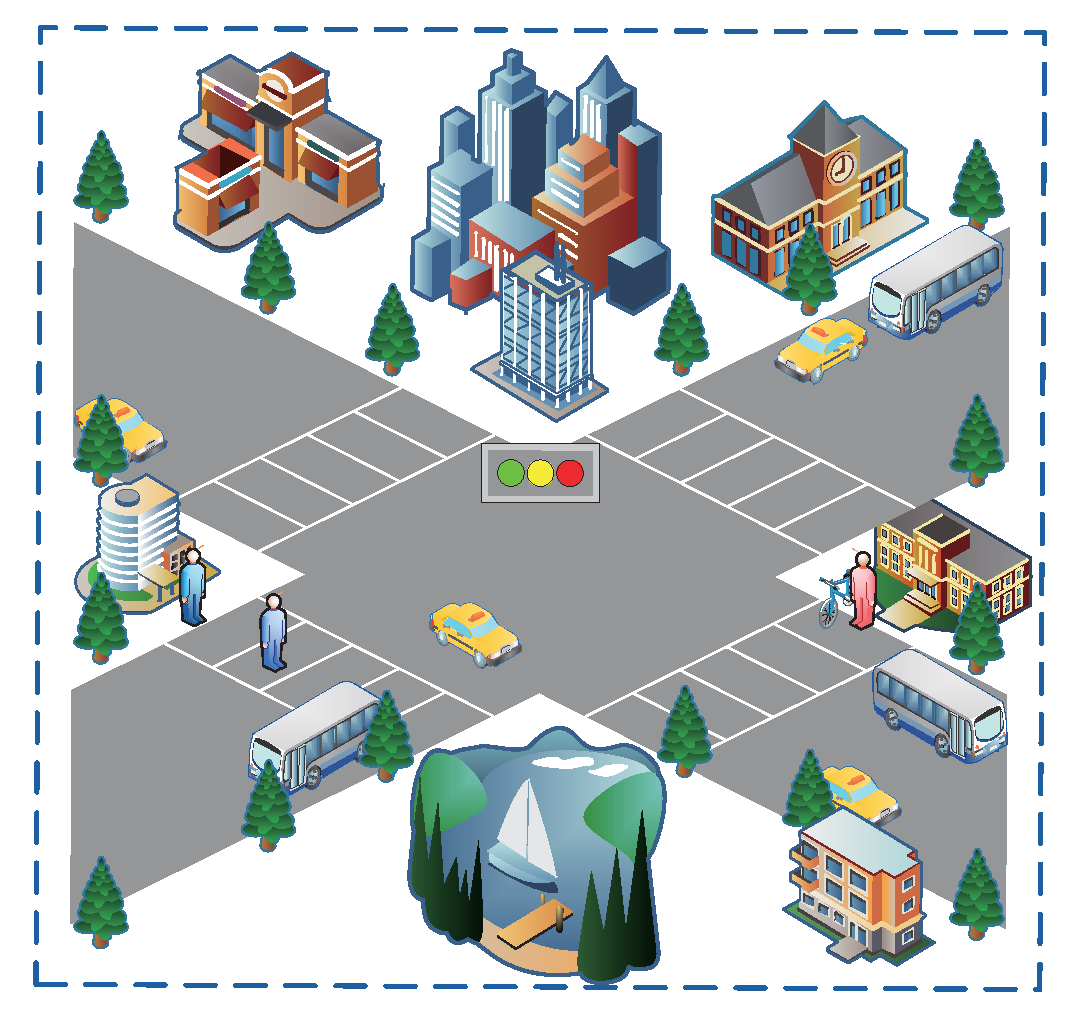
\includegraphics[width=0.8\textwidth]{scenario.eps}
	\caption{场景示意图(五号楷体)}
	\label{chap:scenario}
\end{figure}

图\ref{chap:scenario}展示了xxx。

\begin{figure}[!htb]
	\centering
	\begin{minipage}{0.48\textwidth}
		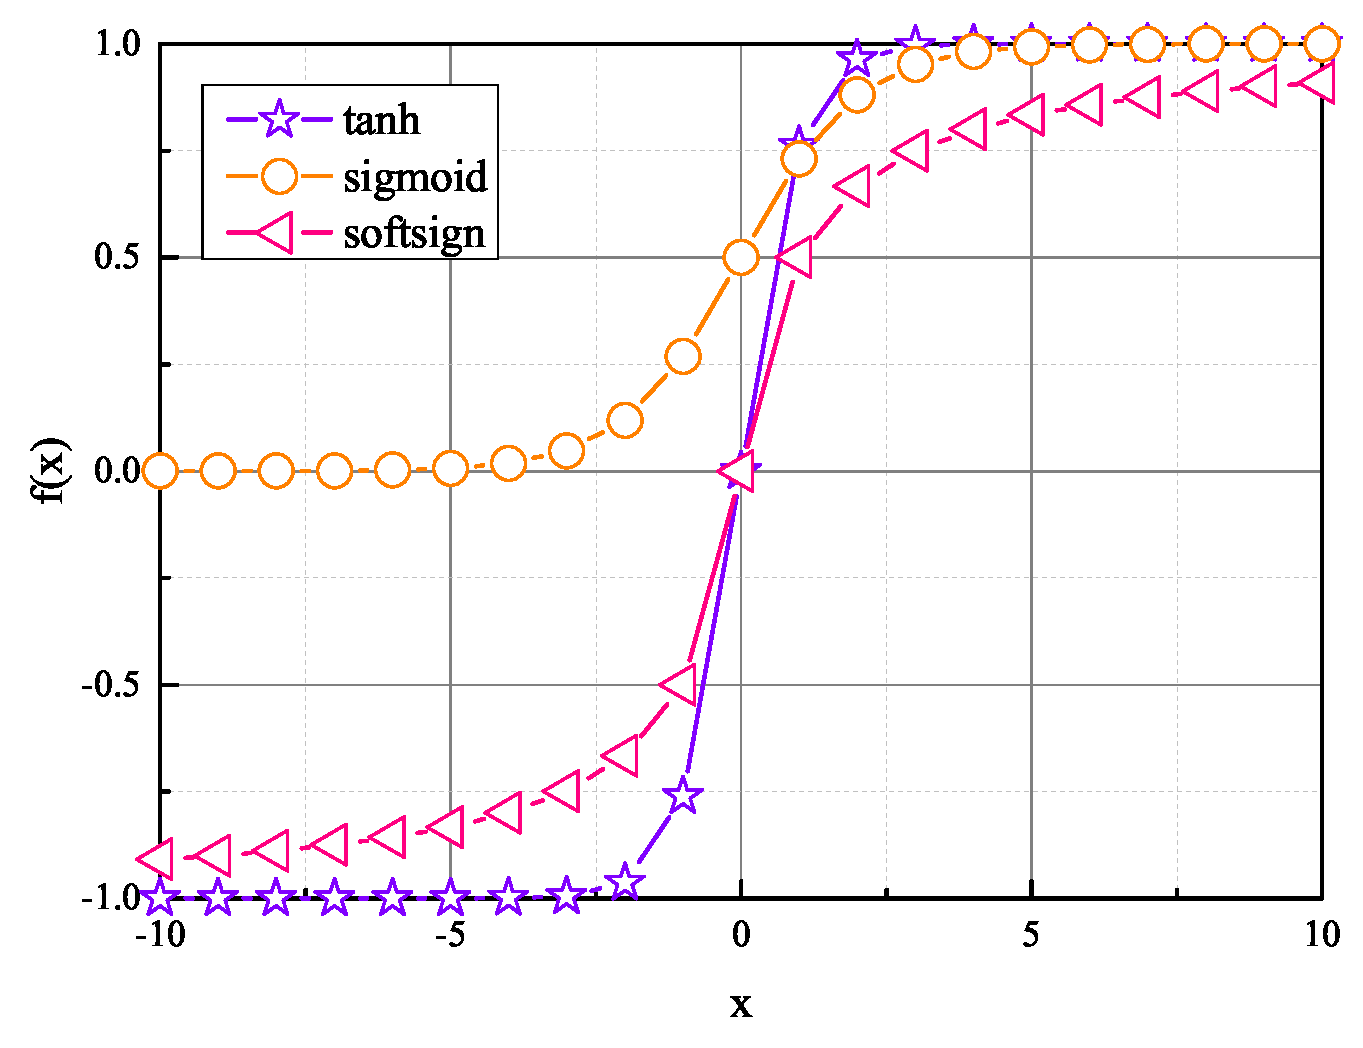
\includegraphics[width=\textwidth]{activation.eps}
		\caption{激活函数}
		\label{chap:activation}
	\end{minipage}
	\begin{minipage}{0.48\textwidth}
		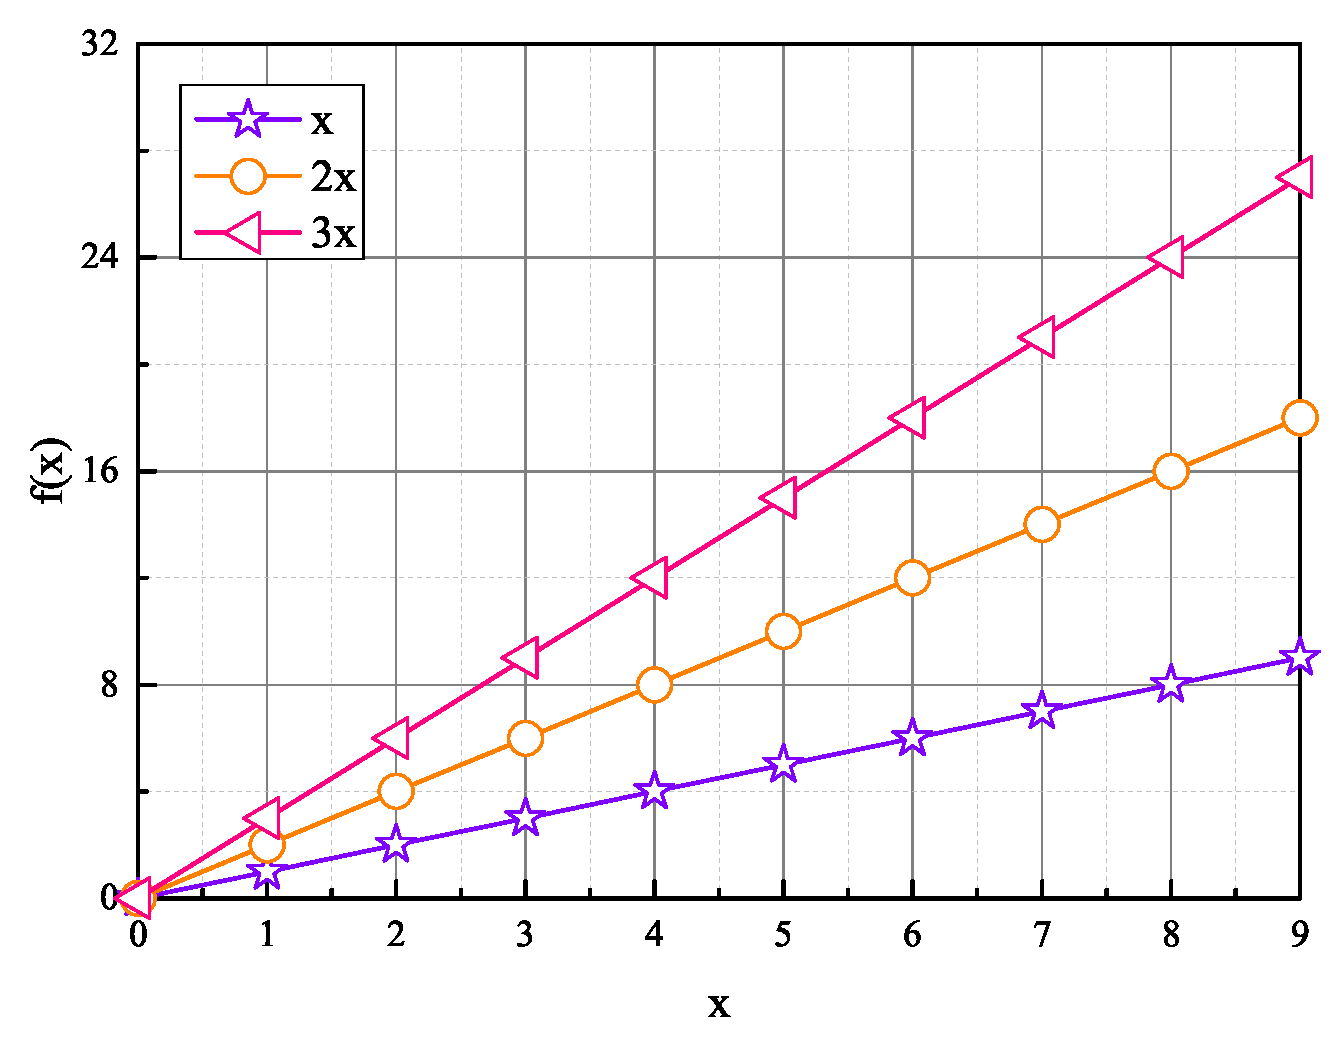
\includegraphics[width=\textwidth]{linear.eps}
		\caption{线性函数}
		\label{chap:linear}
	\end{minipage}
\end{figure}

激活函数\ref{chap:activation},线性函数\ref{chap:linear}


\chapter{算法}

\section{公式}

内联公式:$C = B\log(1 + \gamma)$。

编号公式:

\begin{equation}
J = \frac{1}{2N}\sum(h(x) - y)^2
\end{equation}

\begin{equation}
\nabla J = \frac{1}{N}[\sum(h(x) - y)x]
\end{equation}

\section{算法}

\begin{algorithm}[!htb]
	算法默认采用宏包algorithm2e排版\;
	\BlankLine
	\While{$r < R$} {
		\For{$i = 0$ \KwTo $100$}{
			\If(条件语句可以在这里增加注释){$i = 10$}{
				\lIf{$r = 20$}{$r = r + 1$}
				\tcp{这里可以编写算法注释}
				\lElse{$r\leftarrow i$}
			}
		}
	}
	\caption{algorithm2e算法编写示意}
	\label{chap_algo:example}
\end{algorithm}

引用该算法\ref*{chap_algo:example}。
\bibliography{Bib/thesis}

\backmatter
\BUPTlongestlength{abbreviation = { BUPTBUPTBUPT }}
\begin{abbreviation}
	\item[BUPT] Beijing University of Posts and Telecommunications \hfill 北京邮电大学	
\end{abbreviation}
\begin{acknowledgement}
\LaTeX
\end{acknowledgement}

\begin{publication}
\definecolor{Maroon}{HTML}{701112}
\newcommand{\IF}[1]{\textcolor{Maroon}{(IF = #1)}}
本人攻读学位期间共发表论文1,000篇,其中,第一作者999篇,学生一作1篇,第二作者0篇,其他参与论文共0篇:
\begin{enumerate}
\item XXX, Research on \LaTeX, \emph{Transactions on \LaTeX}, vol. 1, no. 1, Apr. 2019, pp. 0-1. (\IF{100})
\end{enumerate}

发明专利0项


\end{publication}


\end{document}
